\documentclass[12pt,a4paper]{report}
\usepackage[acronym]{glossaries}
\usepackage{datetime}
\usepackage{graphicx}
\usepackage{titling}
\usepackage[nottoc,numbib]{tocbibind}
\usepackage[super]{nth}
\usepackage{url}
\usepackage{listings}
\usepackage{float}
\usepackage{tikz}
\usepackage{fancybox}
\usepackage[htt]{hyphenat}
\usepackage[toc,page]{appendix}
\usepackage{multirow}
\usepackage{siunitx}
\usepackage{pgfgantt}
\usepackage{pgfplots,pgfplotstable}
\usepackage{cite}
\usepackage{microtype}
\usepackage{amssymb}

\pgfplotsset{compat=1.12}

\makeatletter
\newenvironment{CenteredBox}{
\begin{Sbox}}{\end{Sbox}\centerline{\parbox{\wd\@Sbox}{\TheSbox}}}
\makeatother

\usetikzlibrary{positioning,chains,fit,shapes,calc}

\setacronymstyle{long-short}
\loadglsentries{acronyms}
\makenoidxglossaries

\newdate{submissiondate}{03}{05}{2016}
\newdateformat{monthyear}{\monthname[\THEMONTH], \THEYEAR}

\begin{document}

\begin{titlepage}
\centering

\includegraphics[width=0.35\textwidth]{UniOfManchesterLogo}
\par
\vspace{1cm}
{\huge\bfseries Quantified Boolean Formula Solver\par}
\vspace{1cm}
{\Large Solving QBF by converting to EPR\par}
\vspace{2cm}
{\textit{David Green}\par}
{\textit{BSc(Hons) Computer Science and Mathematics}\par}
{\textit{Project report for the third year project under the supervision of Konstantin Korovin in the School of Computer Science at the University of Manchester}\par}
\vfill
{\large \monthyear\displaydate{submissiondate} \par}
\end{titlepage}


\begin{abstract}
This paper details the tool \textit{qbftoepr} that converts \glspl{qbf} to \gls{epr} through a process of Skolemization. This opens new techniques for solving \glspl{qbf} using automated theorem provers for first order logic such as iProver~\cite{korovin2008iprover} over traditional techniques for solving \glspl{qbf} such as (a variation of) the \gls{dpll} algorithm~\cite{davis1962machine}. Other techniques are discussed for improving the efficiency of conversion and reducing the complexity of the \gls{epr} result. In particular, an implementation of dependency schemes is detailed and the concept of anti-prenexing is outlined. The tool is evaluated against the traditional \gls{qbf} solver DepQBF~\cite{lonsing2010depqbf} to compare the efficiency of converting and solving to solving the \gls{qbf} directly. It is also evaluated against another tool called qbf2epr~\cite{seidl2012qbf2epr} that also converts \glspl{qbf} to \gls{epr} to compare it against a different implementation of the same conversion.\newline \newline

\textsc{Acknowledgments}

Thanks to Konstantin Korovin for his help, advice and guidance during the project.
\end{abstract}


\tableofcontents
\newpage

\chapter{Background}
First we must introduce the terminology and concepts of boolean logic including propositional logic, first order logic (including \gls{epr}) and quantified propositional logic.
After the terminology has been introduced the complexity classes of the satisfiability problem of each logic will be discussed.
Finally the concept of automated reasoning of both first order logic and \gls{qbf} will be detailed.

\section{Boolean Logic and Satisfiability}
Boolean logics and \gls{sat} form a calculus which can be used to reason about statements. There are different formal systems of logic that can be used for different purposes, we shall look at propositional logic, \gls{qbf} and first order logic.

\subsection{Propositional Logic}
A propositional variable $p$ can take one of two values; either $true$ or $false$. A variable can be negated using the \gls{not} symbol which reverses its value. If $p$ was $true$ then $\neg p$ is $false$ and vice versa. We will call a variable or its negation a \textit{literal} and denote the positive literal by $l$ and the negative literal by $\bar{l}$.
Boolean formulas are constructed from propositional variables built using the logical connectives \gls{or}, \gls{and} and \gls{implies}. A typical boolean formula might look like $(x \land y) \to z$. A more formal definition can be found in appendix~\ref{formaldefinitions}.

The satisfiability of a boolean formula is a decision problem that asks if an assignment of truth values to propositional variables can make the boolean formula true. The aforementioned logical connectives tell us how to combine the truth values of two variables. With a disjunction, $x \lor y$ is true if either of $x$ or $y$ or both are true. In a conjunction, $x \land y$ is true if both $x$ and $y$ are true. An implication $x \to y$ can be read as ``if $x$ is true then $y$ is true.'' with the case of $x$ being $false$ defined as being vacuously true. In the previous example of $(x \land y) \to z$ we can see that it is satisfiable as the assignment $x := true; y := true; z := true$ makes it true.

We require a more standard form of boolean formula that is easier to describe as an input format. For this we will use \gls{cnf}. \Gls{cnf} is a conjunction of clauses and a clause is a disjunction of literals. For example, a clause might be $(p \lor \neg q)$ and a full formula in \gls{cnf} might look like $(p \lor r) \land (\neg r \lor q) \land (q)$. Using \gls{cnf} allows us to more easily work with boolean formulas algorithmically.

\subsection{Quantified Boolean Formulas} \label{qbf}
\Gls{qbf} extends propositional logic with the \gls{forall} and \gls{exists} quantifiers. The statement $\forall x \exists y (x \lor y)$ states that for every assignment of $x$ there is at least one assignment of $y$ such that the formula $(x \lor y)$ is true. We can see that this \gls{qbf} is satisfiable. If $x := true$ then the formula is true and any assignment of $y$ will work. If $x := false$ then the assignment $y := false$ makes the formula false but the assignment $y := true$ does make the formula true. Therefore, for any assignment of $x$ there exists an assignment of $y$ such that the formula is true. A more formal definition can be found in appendix~\ref{formaldefinitions}.

In the most general case a quantified variable can appear in front of any sub-formula of a \gls{qbf}. Again we need a more standard form of \gls{qbf} that we can deal with algorithmically. This form is called \textit{prenex} \gls{cnf} (however we may refer to it by just \gls{cnf} assuming that the formula is prenexed). Any \gls{qbf} is logically equivalent to a \gls{cnf} formula and the process for transforming the \gls{qbf} into \gls{cnf} is called \textit{prenexing}. This process uses rewriting rules to move all the quantifiers in the formula to the leftmost part of the formula resulting in a \textit{quantifier prefix}. For example, $(\neg (\exists x A) \land B)$ is equivalent to $\forall x (\neg A \land B)$. Because all \glspl{qbf} are equivalent to some \gls{qbf} in \gls{cnf} we shall assume that any \gls{qbf} we are dealing with is already in \gls{cnf}.

Another useful notion will be the idea of an order to a prenexed \gls{qbf}'s prefix. If a variable $x$ is quantified to the left of another variable $y$ in the prefix such as $\exists x \forall y$ we say that $x$ is quantified before $y$. Using this idea we can assign a quantification level to the variables so that $x$ has a quantification level of 1 and $y$ has a quantification level of 2. The variable with the lowest quantification level is called the outermost quantified variable and the variable with the highest quantification level is the innermost.

\subsection{First Order Logic}
First order logic uses propositions that take variables or functions as arguments to form its formulas. These variables range over a specified problem domain such as the natural numbers. For example in the domain of the natural numbers the formula $\forall n \exists m P(n, m)$ where $P(n, m) = m > n$ is true; for any natural number $n$ there is a number $m$ that is larger than $n$. This differs from our previous definition of \gls{qbf} in that \gls{qbf} deals with only variables in a two valued domain (i.e. boolean) and does not have propositions. A more formal definition can be found in appendix~\ref{formaldefinitions}.

Our notions of prenexed \gls{cnf} also extend to first order logic.

As with propositional logic and \gls{qbf} we require a way to write our formulas that is convenient to work with. In this case we will use \gls{epr}, formally known as the \textit{Bernays-Sch{\"o}nfinkel} class of formulas. A formula is in \gls{epr} form if when it is written in \gls{cnf} it has the quantifier prefix $\exists * \forall *$ and contains no functions. This format will be useful because we can solve these problems using first order logic theorem provers.

\section{Complexity of Satisfiability}
Boolean logics are significant in complexity theory as they are standard embeddings for other problems in their complexity classes.

\subsection{SAT is NP-complete}
An NP problem is one that can be solved by a non-deterministic algorithm that runs in time relative to a polynomial of the size of the input. \Gls{sat} is one such problem. Stephen Cook proved in 1971 that the \gls{sat} problem is NP-complete~\cite{cook1971complexity} meaning that any other NP problem can be reduced to the \gls{sat} problem. This spurs lots of interest into \gls{sat} solvers because if we can solve the \gls{sat} problem in polynomial time then we can solve any NP problem in polynomial time too. This is known as the P=NP problem.

\subsection{QBF is PSPACE-complete}
A PSPACE problem is one that can be solved by a deterministic algorithm that runs using space in memory relative to a polynomial of the size of the input. \Gls{qbf} belongs to this complexity class and can be shown to be PSPACE-complete using Savitch's theorem~\cite{savitch1970relationships}. NP problems are a subset of PSPACE problems and it is not yet known if the two classes are equal or not. Because these algorithms run much slower than general \gls{sat} algorithms there has been much less interest in \gls{qbf} solvers outside academia compared to \gls{sat} solvers.

\subsection{EPR is NEXPTIME-complete} \label{eprnexptime}
Similarly to NP problems, NEXPTIME problems are solved by non deterministic algorithms running in time relative to an exponential of the size of the input. \Gls{epr} was shown to be NEXPTIME-complete by Harry Lewis in 1980~\cite{lewis1980complexity}. While this does mean that algorithms for proving satisfiability of \gls{epr} are in general slower than algorithms for propositional satisfiability we are still interested to see how \gls{epr} solvers fare when given inputs derived from \glspl{qbf}.

\section{Automated Reasoning}
Automated reasoning tools use algorithms to solve these \gls{sat} problems as well as other more general logic based problems based around deduction to find a result that isn't necessarily satisfiability. This brings artificial intelligence interests into the research in an effort to create artificial intelligences that can perform deductive reasoning. This project makes use of the automated reasoning tool iProver~\cite{korovin2008iprover} to solve the \gls{sat} problems generated by \textit{qbftoepr}.

\chapter{Converting QBF to EPR} \label{chapter:qbftoepr}
Now that we have introduced the concepts behind \gls{qbf} and \gls{epr} we can look at the procedure that \textit{qbftoepr} implements in greater depth. The algorithm is composed of three main steps detailed below. We shall follow an example through the process from input to output.
The example \gls{qbf} we will work with is formula~\ref{qbf:1}.

\begin{equation} \label{qbf:1}
\begin{aligned}
&\forall w \forall x \forall y \exists z \\
&(y \lor z) &\land\\
&(x \lor \neg z) &\land\\
&(\neg x \lor w)\\
\end{aligned}
\end{equation}

\section{Raising QBF to First Order Logic}
The input to \textit{qbftoepr} is in \gls{qbf} form so it has propositional variables with no notion of predicates. We require an output in first order logic so the inputted \gls{qbf} must be 'raised' to first order logic before the algorithm continues.

This 'raising' is relatively straightforward as most of the symbols used in the \gls{qbf} are also used in first order logic with the only difference being the variables and predicates. For example, the conjunction symbol used in \gls{qbf} can be used in first order logic with the same meaning. To raise the propositional variables used in the clauses to first order logic we introduce a predicate of arity 1 that takes the variable as an argument. For example the propositional variable $x$ would be raised to the predicate $p(x)$. Finally, the predicate $p$ must be defined. This is achieved by adding two clauses $(p(true)) \land (\neg p(false))$ to define how $p$ handles truth values in the new domain. Repeating this process recursively over an inputted \gls{qbf} gives us an \textit{equisatisfiable} formula in first order logic. This means that the \gls{qbf} is satisfiable if and only if the version translated into first order logic is satisfiable.

In the case of the example \gls{qbf}~\ref{qbf:1} raising it to first order logic gives formula \ref{qbf:2}.

\begin{equation} \label{qbf:2}
\begin{aligned}
&\forall w \forall x \forall y \exists z\\
&(p(y) \lor p(z)) &\land\\
&(p(x) \lor \neg p(z)) &\land\\
&(\neg p(x) \lor p(w)) &\land\\
&(p(true)) &\land\\
&(\neg p(false))
\end{aligned}
\end{equation}

\section{Removing Existential Quantifiers by Skolemization} \label{skolemization}
Once we have embedded our \gls{qbf} in first order logic we can begin to turn it into \gls{epr}. This process is called Skolemization~\cite{skolemization}. The first step in this process is to remove the existential quantifiers and replace the variables they quantify with functions (called Skolem functions) that take as arguments the variables that the existential variable 'depends on'. What we mean by 'depends on' will be covered in greater depth in section~\ref{dependencyschemes}. Strictly speaking since \gls{epr} does allow existentially quantified variables at the start of the prefix replacing every existentially quantified variable is not completely necessary but we do require it for the output format. These outermost existential variables will be replaced by constants. Similarly to raising the formula to first order logic this process of Skolemization gives an equisatisfiable formula.

We shall apply Skolemization to our example \gls{qbf}~\ref{qbf:2} after it has been raised to first order logic assuming na{\"i}vely that our existential variables depend on every universal variable. This gives the formula~\ref{qbf:3}.

\begin{equation} \label{qbf:3}
\begin{aligned}
&\forall w \forall x \forall y\\
&(p(y) \lor p(f_z(w, x, y))) &\land\\
&(p(x) \lor \neg p(f_z(w, x, y))) &\land\\
&(\neg p(x) \lor p(w)) &\land\\
&(p(true)) &\land\\
&(\neg p(false))
\end{aligned}
\end{equation}

\section{Removing Function Symbols Introduced by Skolemization}
The final step in converting our \gls{qbf} to \gls{epr} is to remove the function symbols that were introduced by Skolemization. This is done by 'lifting' the functions to predicate. Lifting the functions to predicates means creating a new predicate whose arguments are the variables in the function being lifted. For example $p(f_z(x, y))$ would become the predicate $p_z(x, y)$. Once again this process produces a new formula that is equisatisfiable to the previous formula.

Once all the functions have been lifted to predicates we have our \gls{epr} result. The definition of \gls{epr} required the prefix to be in the form $\exists * \forall *$ which was achieved by Skolemization to remove all the existentially quantified variables and it also required there to be no function symbols which was achieved by lifting the functions to predicates. This result can then be used as the input to an \gls{epr} solver to determine its satisfiability. Because each step in the process preserved satisfiability proving (or disproving) the satisfiability of the \gls{epr} output gives the satisfiability of the original \gls{qbf} input.

Formula~\ref{qbf:4} is formula~\ref{qbf:3} after lifting its functions to predicates.

\begin{equation} \label{qbf:4}
\begin{aligned}
&\forall w \forall x \forall y\\
&(p(y) \lor p_z(w, x, y)) &\land\\
&(p(x) \lor \neg p_z(w, x, y)) &\land\\
&(\neg p(x) \lor p(w)) &\land\\
&(p(true)) &\land\\
&(\neg p(false))
\end{aligned}
\end{equation}

\section{Dependency Schemes} \label{dependencyschemes}
In section~\ref{skolemization} existentially quantified variables were replaced by a function whose arguments were the universally quantified variables that the existentially quantified variable 'depended on'. A dependency scheme maps a variable to the variables that it depends on but this map must be computed. A dependency scheme is called tractable if it can be computed in polynomial time (proportional to the length of the formula). However, the problem of deciding whether a given dependency scheme is the optimal dependency scheme is P-SPACE complete (proved by Marko Samer and Stefan Szeider \cite{backdoorsets}) so it is impractical to compute the optimal dependencies every time.
Dependency schemes are important because they can vastly affect the time to solve a given formula. If the number of variables a variable depends on is reduced the solver does not have to consider all of those extra dependencies and so can solve the formula more quickly.

\subsection{Trivial Dependency Scheme}
The simplest method of assigning dependencies to a variable is to say that it depends on everything that was quantified before it with a different quantifier. For the existentially quantified variables being considered for Skolemization this means that they depend on any variable universally quantified before them. For example in the prefix $\exists w \forall x \forall y \exists z$ the variable $z$ depends on $x$ and $y$ because they were universally quantified before it but not $w$ because it was universally quantified before it. This is called the trivial dependency scheme and is clearly tractable by searching the prefix for universally quantified variables.

\subsection{Standard Dependency Scheme} \label{stddepscheme}
The standard dependency scheme is harder to define so this description will not cover it in great depth. A full description can be found in the aforementioned paper from Samer and Szeider~\cite{backdoorsets}.

We will look at the idea of dependency from the opposite perspective; given a variable, say $x$, what variables depend on $x$? We must first define $R(x)$ to be the all the existential variables quantified to the right of $x$. Then we have a notion of dependency pairs in which two variables $x$ and $y$ (with $y$ quantified to the right of $x$) form a dependency pair $(x,y)$ if they are 'connected' with respect to $R(x)$. The two variables $x$ and $y$ are connected with respect to $R(x)$ if in the incidence graph of the formula there exists a path through the graph from a clause containing $x$ to a clause containing $y$ that only travels through clauses that contain at least one variable in $R(x)$. The incidence graph is a bipartite graph with a variable joined to a clause if the variable is in the clause. A path starts at one clause, travels to a variable in $R(x)$ and from that variable travels to a clause and so on until it reaches a clause containing $y$. Trivially, if $x$ and $y$ are in the same clause then $y$ depends on $x$.

Figure~\ref{bigrapheasy} is the incidence graph of formula~\ref{qbf:1}. Trivially we can see that $z$ depends on both $x$ and $y$ because it appears in clauses with both of them but compared to the trivial dependency scheme it hasn't given $w$ as a dependency of $z$ because there is no path from $w$ to $z$ in the graph traveling only through clauses containing variables in the set $R(w)=\left \{z\right \}$, the only way to do so is to go via $x$ which is not in $R(w)$. Despite being quantified to the right of $w$, $x$ was quantified universally so it is not included.

\begin{figure}
\begin{CenteredBox}
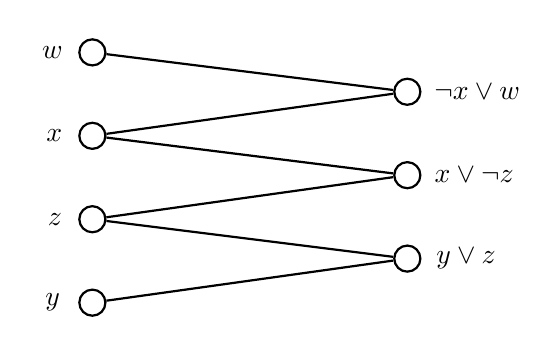
\begin{tikzpicture}[
thick,
every node/.style={draw,circle},
]

\begin{scope}[start chain=going below,node distance=7mm]
\node[on chain] (lw) [label=left: $w$] {};
\node[on chain] (lx) [label=left: $x$] {};
\node[on chain] (lz) [label=left: $z$] {};
\node[on chain] (ly) [label=left: $y$] {};
\end{scope}

\begin{scope}[xshift=4cm,yshift=-0.5cm, start chain=going below, node distance=7mm]
\node[on chain] (c1) [label=right: $\neg x \lor w$] {};
\node[on chain] (c2) [label=right: $x \lor \neg z$] {};
\node[on chain] (c3) [label=right: $y \lor z$] {};
\end{scope}

\draw (lw) -- (c1);
\draw (lx) -- (c1);
\draw (lx) -- (c2);
\draw (lz) -- (c2);
\draw (lz) -- (c3);
\draw (ly) -- (c3);

\end{tikzpicture}

\end{CenteredBox}
\caption{Bipartite graph for formula~\ref{qbf:1}}
\label{bigrapheasy}
\end{figure}

To see less obvious dependencies with the standard dependency scheme we need a slightly more complex example. Consider formula~\ref{hardformula}.

\begin{equation}
\label{hardformula}
\begin{aligned}
&\forall u \exists v \forall w \exists x \forall y \exists z\\
&(u \lor \neg v \lor x) &\land\\
&(u \lor \neg x) &\land\\
&(v \lor z) &\land\\
&(v \lor \neg z) &\land\\
&(w \lor x \lor y) &\land\\
&(y \lor \neg z)\\
\end{aligned}
\end{equation}

The graph for formula~\ref{hardformula} is figure~\ref{bigraphhard}.

\begin{figure}
\begin{CenteredBox}
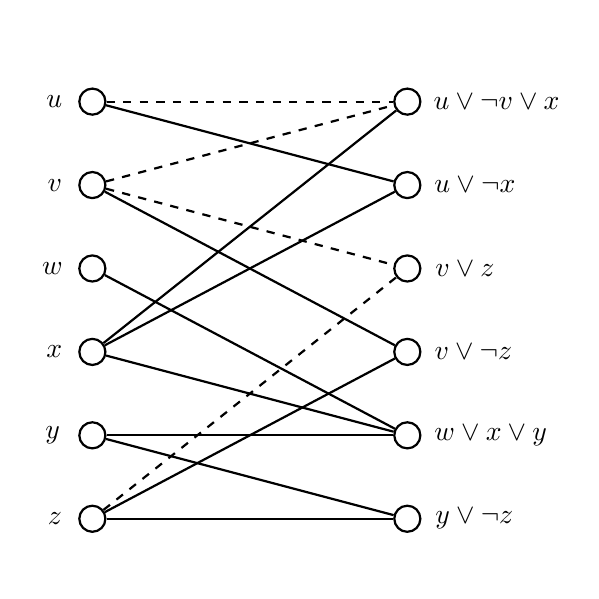
\begin{tikzpicture}[
thick,
every node/.style={draw,circle},
]

\begin{scope}[start chain=going below,node distance=7mm]
\node[on chain] (lu) [label=left: $u$] {};
\node[on chain] (lv) [label=left: $v$] {};
\node[on chain] (lw) [label=left: $w$] {};
\node[on chain] (lx) [label=left: $x$] {};
\node[on chain] (ly) [label=left: $y$] {};
\node[on chain] (lz) [label=left: $z$] {};
\end{scope}

\begin{scope}[xshift=4cm,start chain=going below,node distance=7mm]
\node[on chain] (c1) [label=right: $u \lor \neg v \lor x$] {};
\node[on chain] (c2) [label=right: $u \lor \neg x$] {};
\node[on chain] (c3) [label=right: $v \lor z$] {};
\node[on chain] (c4) [label=right: $v \lor \neg z$] {};
\node[on chain] (c5) [label=right: $w \lor x \lor y$] {};
\node[on chain] (c6) [label=right: $y \lor \neg z$] {};
\end{scope}

\draw[dashed] (lu) -- (c1);
\draw (lu) -- (c2);
\draw[dashed] (lv) -- (c1);
\draw[dashed] (lv) -- (c3);
\draw (lv) -- (c4);
\draw (lw) -- (c5);
\draw (lx) -- (c1);
\draw (lx) -- (c2);
\draw (lx) -- (c5);
\draw (ly) -- (c5);
\draw (ly) -- (c6);
\draw[dashed] (lz) -- (c3);
\draw (lz) -- (c4);
\draw (lz) -- (c6);

\end{tikzpicture}

\end{CenteredBox}
\caption{Bipartite graph for formula~\ref{hardformula}}
\label{bigraphhard}
\end{figure}

It is not obvious from the formula that under the standard dependency scheme that $z$ depends on $u$. However in this case $R(u)=\left \{v, x, z\right \}$ and a path starting at the clause $(v \lor z)$ can travel through $v$ (because it is in $R(u)$) and thus reach the clause $(u \lor \neg v \lor x)$ which contains $u$. This is the path labeled in dashed lines on the graph. We can also see that $z$ does not depend on $w$ as a path to $w$ must travel through $x$ or $y$, neither of which are in $R(w)$.

The standard dependency scheme is tractable (full proof by Samer and Szeider~\cite{backdoorsets}) because we can work backwards from a given variable $x$ to see what variables depend on it doing a linear search across the graph and upon finding a variable that matches the criteria it is added to the list of variables that depend on $x$. 

\chapter{Development}
\todo[inline]{Development goes here}
This chapter will describe the design and implementation of \textit{qbftoepr} at a high level with some of the technical choices and why they were made as well as some of the optimizations and compromises that were taken to improve performance.

\section{Language Choice}
The project was implemented in the language OCaml~\cite{ocaml} which is a functional language notable for the language extensions that give it object oriented and imperative functionality. The main motivator for implementing \textit{qbftoepr} in OCaml is the fact that iProver is implemented in OCaml which provides three advantages:

\begin{itemize}
\item Code from iProver can be re-used easily in \textit{qbftoepr}\\
\item Using the same language in \textit{qbftoepr} as iProver makes post-project maintenance easier\\
\item Using the same language would allow tighter integration when \textit{qbftoepr} passes its output to iProver (though this wasn't done in practice)\\
\end{itemize}

Even without these advantages OCaml would be a suitable language given that it has been designed with performance as a priority and has excellent built-in functions for manipulating lists of which the project makes extensive use.

\section{Input and Output Formats}
The input and output formats were an important choice but one that was relatively easy to make. The decision was to go with the standards already in use by other theorem provers to be able to compare \textit{qbftoepr} to them on exactly the same inputs. Another consideration was that the input format had to have a relatively simple grammar to simplify the input handling and the output format had to be simple enough to make printing the output efficient. The output format must also be accepted as an input format by iProver.

\subsection{QDIMACS}
QDIMACS~\cite{qdimacs} is the input format decided on for \textit{qbftoepr}. It is the format used by the QBFLIB~\cite{qbflib} which is a library of \gls{qbf} problem instances. QBFLIB also holds a competition called QBFEVAL which tests \gls{qbf} solvers against each other using the QDIMACS format. This makes it the standard of the \gls{qbf} research community and a clear choice of input format for \textit{qbftoepr}. It also opens access to the QBFLIB problem library providing test cases of all difficulty scales and the results of other solvers on these test cases. It also has a very simple grammar meaning that parsing a QDIMACS input is simple.

Below is our example from chapter~\ref{chapter:2} in QDIMACS form.
\begin{lstlisting}
c this is a comment
p cnf 4 3
a 1 2 3 0
e 4 0
3 4 0
2 -4 0
-2 1 0
\end{lstlisting}
Lines beginning with \textit{c} are comments, \textit{p} denotes the problem line which tells us the problem is in \gls{cnf} and has four variables and three clauses. Lines prefixed with \textit{a} are universally quantified variables, \textit{e} are existential. Lines after the prefix form the matrix which is the list of clauses. Numbers represent variables and a negative number represents the negative literal of that variable, i.e. $\bar{l}$. The prefix and matrix lines are appended with a zero as a line terminator.

\subsection{TPTP}
The output format chosen for \textit{qbftoepr} is TPTP~\cite{tptp}. Similarly to QBFLIB, the TPTP is a large problem library for automated theorem proving and as such it is one of the input formats that iProver accepts. The popularity of the TPTP library means it is also used by other automated theorem provers. Because the TPTP is a general problem library (whereas QBFLIB is specifically \gls{qbf} problems) its grammar is very complicated. However \textit{qbftoepr} does not need to parse it to output it and only requires a small subset of the format's features to output the result of the \gls{epr} conversion process.

Below is the example from chapter~\ref{chapter:2} after being converted to \gls{epr} in the TPTP output format.
\begin{lstlisting}
cnf(cl_0,plain,(p(X3) | p_f_4(X1,X2,X3))).
cnf(cl_1,plain,(p(X2) | ~p_f_4(X1,X2,X3))).
cnf(cl_2,plain,(~p(X2) | p(X1))).
cnf(cl_3,plain,(p(true))).
cnf(cl_4,plain,(~p(false))).
\end{lstlisting}
Each line is a clause, named \textit{cl\_x} where x is an identifier. Following is the \textit{plain} keyword which says there are no user defined semantics then the list of literals where \textit{\textasciitilde} denotes the negation of a literal.

\section{Data Structures}

\section{Implementation}
\subsection{Skolemization}
\subsection{Removing Functions}
\subsection{Dependency Scheme Construction}
\subsection{Complexity}
% raising to fol is linear in the number of clauses (and in their length?)? just translate symbols one at a time plus two extra clauses but that's dominated by the linearity of the symbol translation
% skolemization: finding existential variables linear in the length of the prefix n, then one linear search of the matrix for each variable found, another n*m? (n*m)^2? disclaimer this might be wrong
% removing functions is linear in the number of clauses (and in their length?)? replacing functions with predicates one by one

\section{Optimizations}

\section{Future Work}
\subsection{Dependency Scheme Optimizations}
\subsection{Anti-prenexing}

\chapter{Evaluation} \label{evaluation}
This chapter discusses the evaluation of \textit{qbftoepr} starting with the automated testing to determine the functionality is correct then benchmarks against other \gls{qbf} solvers and also against \textit{qbf2epr}, a tool that also converts \gls{qbf} to \gls{epr}.

\section{Automated Testing}
Automated testing was implemented using the OUnit library which is an OCaml analogue of JUnit for Java. Each function was tested individually against valid and invalid inputs to determine whether the code behaved correctly then linked together in integration tests to test the sections of the algorithm (such as Skolemization) from the top level. Each update to the code also updated the tests if required and ensured that the tests were passing before the code was committed.

\section{Testing Methodology}
Two test sets were selected from the QBFLIB 2010 problem library. The first was an easy set consisting of four easier problems with fewer clauses and the second was a more difficult set of sixteen harder problems with orders of magnitude more clauses. The exact problems are listed in appendix~\ref{qbfproblemsets}.

The easy set was used to test \textit{qbftoepr} against the \gls{qbf} solver DepQBF. The problems generated by the harder set were not practical to solve using iProver due to time constraints. This will become evident when comparing the iProver solving time of results generated using the trivial dependency scheme versus the standard in subsection~\ref{tvsstdsolve}. The easy set of benchmarks runs quickly enough to be able to benchmark efficiently but is complex enough to still provide a useful benchmark.

The hard set is used when evaluating the different dependency schemes and when comparing \textit{qbftoepr} to \textit{qbf2epr}. The solving time of iProver doesn't matter when comparing the two \gls{epr} converters because they produce the same result (ignoring differences in naming of variables and predicates) so a harder data set can be used to really challenge the converters.

The tests were run on a mid-2014 Macbook Pro with an Intel Core i7-4578U processor and 16GB of 1600MHz RAM running OS X El Capitan version 10.11.4. Each benchmark was ran three times to take an average.

\section{Comparison Between Trivial and Standard Dependency Schemes} \label{trivialvsstd}
Because the implementation of the standard scheme is inefficient it is expected to take much longer to convert the \gls{qbf} than the trivial scheme. The real benefits of the standard scheme are shown in the size of the outputted \gls{epr} result as a smaller output from the same input indicates the variable dependencies that were removed. This small result then follows into less time taken for iProver to solve the result. The exact results of this testing can be found in appendix~\ref{trivialvsstandardappendix}.

\subsection{Time Taken to Convert}
As expected using the standard dependency scheme means the conversion takes significantly more time on larger problem instances. The difference is much larger for larger problem sets. This is most clear by looking at the ratio of time taken to convert using the standard scheme over the time taken to convert using the trivial scheme as the number of clauses in the problem increases. In the smallest cases the trivial scheme might only be twice as fast but on the largest problems it can be forty times as fast. There is a linear relationship between this ratio and the number of clauses in the problem. Roughly doubling the number of clauses roughly doubles the ratio of trivial time over standard time.

\begin{center}
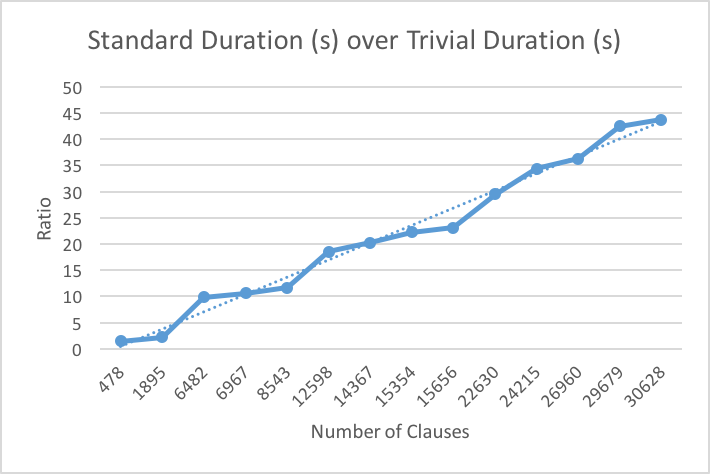
\includegraphics{standarddurationovertrivialduration.png}
\end{center}

\subsection{Size of Result}
The standard scheme does produce significantly smaller results than the trivial scheme. The relationship is similar to that in the time taken to convert with the inverse ratio. We look at the ratio of the size of the trivial scheme result over the size of the standard scheme result. In the smallest cases the standard scheme is at least four to five times smaller but can be as much as two hundred times smaller for larger problems. Again there is a linear relationship between the number of clauses and this ratio. As the number of clauses doubles, the ratio of trivial size over standard size doubles too.

\begin{center}
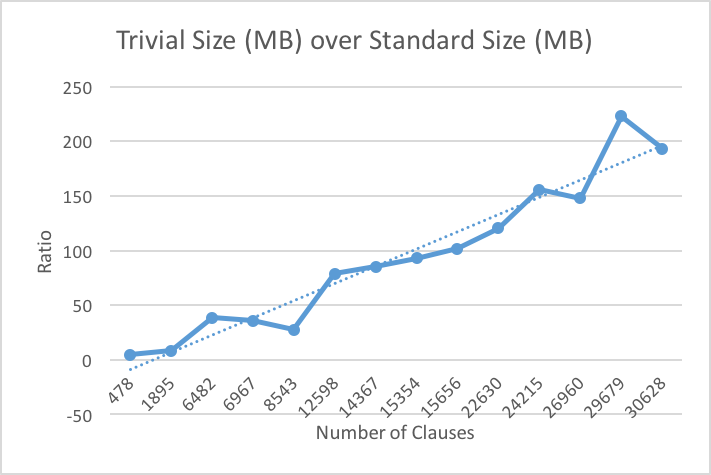
\includegraphics{trivialsizeoverstandardsize.png}
\end{center}

Given that this implementation of the standard dependency scheme misses some dependencies the correct file size is slightly higher but not enough to break this relationship.

\subsection{Time to Solve} \label{tvsstdsolve}
The hope is that the smaller problems are faster for iProver to solve and that this speed improvement outweighs the deficit introduced by the longer conversion time. This proved to be harder to show but can be loosely inferred from a single result. The problem \texttt{s27\_d5\_u-shuffled} is the smallest problem in the harder data set with 478 clauses. Using the trivial scheme took 0.015 seconds to convert to \gls{epr} with an output file-size of 117 Kilobytes and using the standard scheme took 0.021 seconds with an output of 26 Kilobytes. However, iProver took only 147.12 seconds to solve the standard result but had not solved the trivial result after an hour of processing. This shows that the extra time taken to convert using the standard dependency scheme is vastly outweighed by the time taken to solve in iProver on sufficiently large problems. To test this inference further the same test was carried out using the easy set of benchmarks but the difference here was negligible on the easy problems with only a hundred clauses.

\section{Comparison Against a Direct QBF Solver}
As mentioned to in section~\ref{eprnexptime}, in theory solving \gls{epr} is slower than solving the \gls{qbf} directly. The results agreed with this theory. Solving via converting with \textit{qbftoepr} and solving the \gls{epr} with iProver was approximately an order of magnitude slower than solving the problem directly with DepQBF. The full results can be seen in appendix~\ref{depqbfvsqbftoepr}. 

\begin{center}
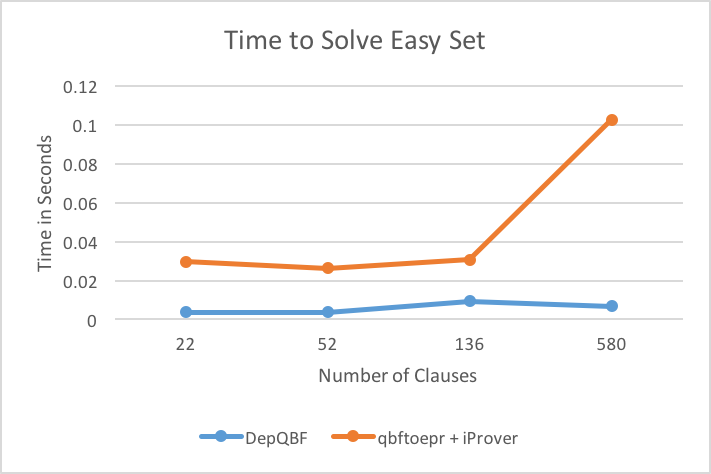
\includegraphics{depqbfvsqbftoepr.png}
\end{center}

\section{Comparison Against an EPR Converter}
The trivial dependency scheme is used throughout these tests as it is the only scheme implemented in qbf2epr so it is used when testing \textit{qbftoepr} to give a better comparison. Since the two converters give identical output (aside from differences in variable names) only the conversion time is examined as the differences in time taken for iProver to solve the output would be negligible. The results show that the conversion time of qbf2epr increases linearly with the number of clauses whereas \textit{qbftoepr} increases with the square of the number of clauses. This means that as the problem size increases the algorithmic inefficiencies in \textit{qbftoepr} lead to a significant time difference, up to 20 times slower in the largest problem. However on the smaller problem sets \textit{qbftoepr} is almost an order of magnitude faster than qbf2epr suggesting that if it were improved it could be significantly faster on larger problem sets.

\begin{center}
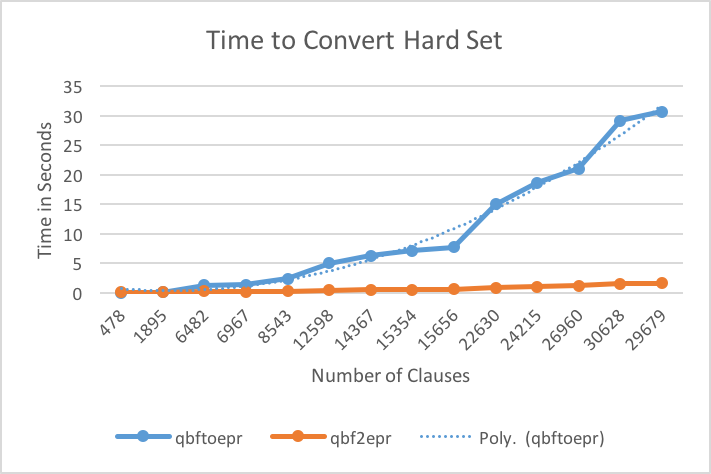
\includegraphics{qbftoeprvsqbf2eprhard.png}
\end{center}

\begin{center}
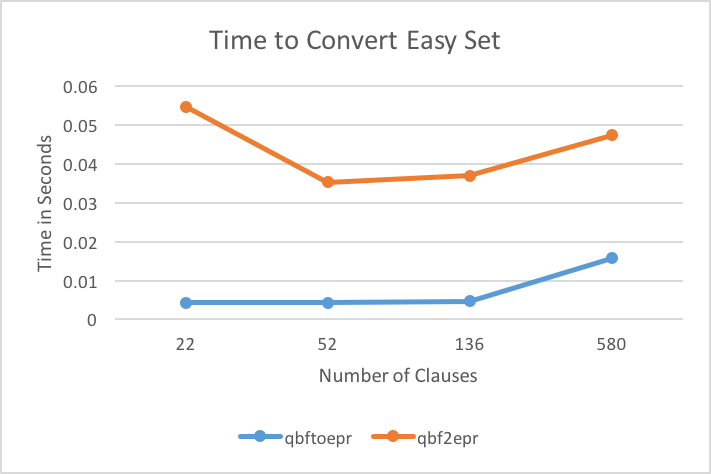
\includegraphics{qbftoeprvsqbf2epreasy.png}
\end{center}

\chapter{Future work}
\todo[inline]{Future work goes here}

\section{Dependency Scheme Optimisations}

\section{Anti-prenexing}

\chapter{Conclusion}
Finally, this chapter will summarize the project first looking at the progress then some closing analysis.

\section{Progress}
The project progressed slowly at first. The mix of multiple new technologies to learn at once delayed the start of the project until it was roughly six weeks behind. However from the implementation of Skolemization the project proceeded according to plan until the project demo. At this stage the project was extremely inefficient and not in a suitable state for providing evaluation results for the project demo. This meant that time had to be spent on improving the basic functionality rather than implementing some of the extensions that were originally planned beyond just the standard dependency scheme. The gantt chart in appendix~\ref{ganttchart} shows the planned time for each stage of the development.

\section{Conclusion}
The aim of the project was to produce a tool that would take a \gls{qbf} as input and produce an \gls{epr} output to be used in iProver. This was completed in the estimated time frame with extensions to the original functionality to use the standard dependency scheme over just the trivial dependency scheme. Some extensions such as the triangle dependency scheme and anti-prenexing discussed in chapter~\ref{futurework} were not implemented due to time constraints. It does not perform as well as competing tools but with more time the implementation could be improved to the point where it would be faster than the competing tools.

Overall the project was a valuable learning experience from the first experiences with a functional language to researching beyond the undergraduate course to understand the background of the project.


\bibliography{bibl}
\bibliographystyle{plain}

\printnoidxglossaries

\begin{appendices}
\chapter{Formal Definitions} \label{formaldefinitions}

\section{Propositional Logic}
First define the language $\mathcal{L}(A, \Omega, Z, I)$. The set $A$ is the alphabet; the set of variables that can be used in formulas. The set $\Omega$ is the set of operators of various arities. The set $Z$ is the inference rules and $I$ is the set of logical axioms.

Formulas are defined by saying that any element of $A$ is a formula and if $p_1,p_2,\dotsc,p_n$ are formulas and $f \in \Omega$ is a logical operator of arity $n$ then $f(p_1,p_2,\dotsc,p_n)$ is a formula.

\section{QBF}
The definition of a formula in \gls{qbf} is similar to that of propositional logic however a set $\phi$ is introduced containing the quantifiers. In this case we will consider $\phi=\left \{\exists, \forall\right \}$. 

As in propositional logic, formulas are defined by saying that any element of $A$ is a formula and if $p_1,p_2,\dotsc,p_n$ are formulas and $f \in \Omega$ is a logical operator of arity $n$ then $f(p_1,p_2,\dotsc,p_n)$ is a formula but also if $p$ is a formula, $Q \in \phi$ is a quantifier and $x \in A$ is a variable then $Qx p$ is a formula.

\section{First Order Logic}
First order logic introduces predicates which makes the definition more complicated than that of propositional logic. There is a set $\mathcal{V}$ of variables, a set $\mathcal{C}$ of constants, $\mathcal{F}$ of functions, $\mathcal{R}$ a set of relation symbols and the logical symbols $\neg, \to, \forall$. 

A term is defined as an element of $\mathcal{V} \cup \mathcal{C}$ and if $t_1,t_2,\dotsc,t_n$ are terms and $f\in\mathcal{F}$ is a function of arity $n$ then $f(t_1,t_2,\dotsc,t_n)$ is a term.

To define formulas we first define a relation, if $t_1,t_2,\dotsc,t_n$ are terms and $R\in\mathcal{R}$ is a relation of arity $n$ then $R(t_1,t_2,\dotsc,t_n)$ is a formula. More complex formulas are then built up using the logical symbols. If $\varphi$ and $\psi$ are formulas and $x$ is a variable then $(\neg\varphi)$, $(\varphi\to\psi)$ and $(\forall x\phi)$ are formulas.

The more familiar connectives of $\lor$ and $\land$ and the quantifier $\exists$ can be made out of these logical symbols. The formula $\varphi\lor\psi$ is logically equivalent to $(\neg\varphi)\to\psi$, the formula $\varphi\land\psi$ is logically equivalent to $\neg(\varphi\to(\neg\psi))$ and the formula $\exists x \varphi$ is logically equivalent to $\neg\forall x(\neg\varphi)$.

\chapter{Code Listings} \label{codelistings}

\section{Factorial Example}

\begin{figure}[H]
\caption{Factorial example}
\begin{CenteredBox}
\begin{lstlisting}[language=caml, label=ocamlex]
let rec factorial n =
  if n <= 1 then 1
  else n * factorial (n - 1)
\end{lstlisting}

\end{CenteredBox}
\end{figure}

\section{QDIMACS Example}

\begin{figure}[H]
\caption{QDIMACS example}
\begin{CenteredBox}
\begin{lstlisting}[label=qdimacsex]
c this is a comment
p cnf 4 3
a 1 2 3 0
e 4 0
3 4 0
2 -4 0
-2 1 0
\end{lstlisting}

\end{CenteredBox}
\end{figure}

\section{TPTP Example}

\begin{figure}[H]
\caption{TPTP example}
\begin{CenteredBox}
\begin{lstlisting}[label=tptpex]
cnf(cl_0,plain,(p(X3) | p_f_4(X1,X2,X3))).
cnf(cl_1,plain,(p(X2) | ~p_f_4(X1,X2,X3))).
cnf(cl_2,plain,(~p(X2) | p(X1))).
cnf(cl_3,plain,(p(true))).
cnf(cl_4,plain,(~p(false))).
\end{lstlisting}

\end{CenteredBox}
\end{figure}

\section{Raising to First Order Logic}

\begin{figure}[H]
\caption{Raising to first order logic}
\begin{CenteredBox}
\begin{lstlisting}[language=caml, label=raisingtofol]
let convert_qbf_to_fol qbf =
  {prefix = convert_qbf_prefix_to_fol qbf.qbf_prefix;
   matrix = 
     convert_matrix_to_fol qbf.qbf_matrix 
     @ clauses_for_introduced_predicate}

let convert_matrix_to_fol qbf_matrix =
  List.map convert_clause_to_fol qbf_matrix

let convert_clause_to_fol clause =
  List.map convert_literal_to_fol clause

let convert_literal_to_fol literal =
  match literal.sign with
    Pos -> make_pos_literal 
      (make_predicate fol_pred_name [Atom(literal.atom)])
  | Neg -> make_neg_literal 
      (make_predicate fol_pred_name [Atom(literal.atom)])
\end{lstlisting}

\end{CenteredBox}
\end{figure}

\section{Skolemization}

\begin{figure}[H]
\caption{Skolemization}
\begin{CenteredBox}
\begin{lstlisting}[language=caml, label=skolemizationimpl]
let skolemization fol_qbf dep_scheme =
  let skolem_list = build_skolem_func_list fol_qbf.prefix dep_scheme in
  build_fol_qbf
  (prefix_without_existential_variables fol_qbf.prefix)
  (get_skolemized_matrix fol_qbf.matrix skolem_list)

let rec build_skolem_func_list prefix dep_scheme =
  try
    let outermost = List.find (fun var -> var.quantifier = E) prefix in
    let func_args = List.assoc outermost.atom dep_scheme in
    [outermost.atom, build_skolem_function outermost func_args]
    @ (build_skolem_func_list 
        (prefix_without_quantifier prefix outermost) 
        dep_scheme)
  with Not_found -> []

let get_skolemized_matrix matrix skolem_list =
  List.map (get_skolemized_clause skolem_list) matrix

let get_skolemized_clause skolem_list clause =
  List.map (get_skolemized_literal skolem_list) clause

let get_skolemized_literal skolem_list literal =
  {sign = literal.sign; 
   pred = get_skolemized_predicate skolem_list literal.pred}

let get_skolemized_predicate skolem_list predicate =
  let atom = List.hd predicate.pred_arguments in
  match atom with
    Atom(n) ->
      make_predicate
      predicate.pred_name
      (replace_atom_with_skolem_func n skolem_list)
  | _ -> predicate
\end{lstlisting}

\end{CenteredBox}
\end{figure}

\section{Removing Functions}

\begin{figure}[H]
\caption{Removing Functions}
\begin{CenteredBox}
\begin{lstlisting}[language=caml, label=removingfunctionsimpl]
let remove_functions_from_fol_qbf fol_qbf =
  let new_matrix = remove_functions_from_matrix fol_qbf.matrix in
  build_fol_qbf fol_qbf.prefix new_matrix

let remove_functions_from_matrix matrix =
  List.map remove_functions_from_clause matrix

let remove_functions_from_clause clause =
  List.map remove_function_from_literal clause

let remove_function_from_literal literal =
  {sign = literal.sign; 
   predicate = remove_function_from_predicate literal.predicate}

let remove_function_from_predicate predicate =
  match List.hd predicate.predicate_arguments with
    Func(f) -> raise_function_to_predicate f
  | _ -> predicate
\end{lstlisting}

\end{CenteredBox}
\end{figure}

\section{Trivial Dependency Scheme}

\begin{figure}[H]
\caption{Trivial Dependency Scheme}
\begin{CenteredBox}
\begin{lstlisting}[language=caml, label=trivialdepschemeimpl]
let universally_quantified_below_quant_level prefix quant_level =
  List.filter (universally_quantified_before quant_level) prefix

let universally_quantified_before quant_level var =
  var.quantifier = A && var.quant_level < quant_level
\end{lstlisting}

\end{CenteredBox}
\end{figure}

\section{Standard Dependency Scheme}

\begin{figure}[H]
\caption{Standard Dependency Scheme}
\begin{CenteredBox}
\begin{lstlisting}[language=caml, label=stddepschemeimpl]
let std_dep_scheme_for_variable qbf var =
  let all_potential_atoms =
   List.sort_uniq
     compare_atoms
     (atoms_of_clauses (clauses_containing_atom var.variable qbf.matrix)) in
  [var.variable,
   List.filter
     (universally_quantified_before_variable qbf.prefix var)
     all_potential_atoms]

let universally_quantified_before_variable prefix var_one atom_two =
  let quant_var_two = quantified_variable_for_atom atom_two prefix in
  universally_quantified_before var_one.quant_level quant_var_two

let clause_contains_atom atom clause =
  List.exists (fun literal -> literal.atom = atom) clause

let clauses_containing_atom atom matrix =
  List.filter (clause_contains_atom atom) matrix
\end{lstlisting}

\end{CenteredBox}
\end{figure}

\chapter{QBF Problem Sets} \label{qbfproblemsets}

Append \texttt{-shuffled.qimacs} for the filename in the QBFLIB 2010 set.

\section{Easy Set}

\begin{center}
\begin{tabular}{| l | S[table-format=3.2] | S[table-format=3.2] |}
\hline
\textbf{Name} & \textbf{No. Variables} & \textbf{No. Clauses} \\ \hline
\texttt{toilet\_g\_02\_01.2} & 11 & 22 \\
\texttt{toilet\_g\_04\_01.2} & 22 & 52 \\
\texttt{toilet\_g\_08\_01.2} & 43 & 136 \\
\texttt{toilet\_g\_20\_01.2} & 105 & 580 \\
\hline
\end{tabular}
\end{center}

\section{Hard Set}

\begin{center}
\begin{tabular}{| l | S[table-format=3.2] | S[table-format=3.2] |}
\hline
\textbf{Name} & \textbf{No. Variables} & \textbf{No. Clauses} \\ \hline
\texttt{s1196\_d3\_u} & 7758 & 14367 \\
\texttt{s1269\_d3\_s} & 8353 & 15354 \\
\texttt{s27\_d5\_u} & 403 & 478 \\
\texttt{s298\_d11\_s} & 22003 & 15656 \\
\texttt{s298\_d2\_s} & 853 & 1895 \\
\texttt{s298\_d5\_s} & 4744 & 6482 \\
\texttt{s298\_d9\_s} & 14846 & 12598 \\
\texttt{s386\_d12\_u} & 36462 & 24215 \\
\texttt{s499\_d15\_s} & 56827 & 30628 \\
\texttt{s499\_d4\_s} & 4368 & 6967 \\
\texttt{s510\_d12\_s} & 45786 & 29679 \\
\texttt{s510\_d4\_s} & 5506 & 8543 \\
\texttt{s820\_d6\_s} & 18299 & 22630 \\
\texttt{s820\_d7\_s} & 24757 & 26960 \\
\hline
\end{tabular}
\end{center}

\chapter{Trivial vs. Standard Dependency Scheme} \label{trivialvsstandardappendix}

\section{Trivial Results}

\begin{center}
\begin{tabular}{| l | S[table-format=3.2] | S[table-format=3.2] |}
\hline
\textbf{Name} & \textbf{Average Time in Seconds} & \textbf{Result Filesize in Bytes} \\ \hline
\texttt{s1196\_d3\_u} & 6.2243 & 75655431 \\
\texttt{s1269\_d3\_s} & 7.0686 & 87889943 \\
\texttt{s27\_d5\_u} & 0.0150 & 120032 \\
\texttt{s298\_d11\_s} & 7.7326 & 105460769 \\
\texttt{s298\_d2\_s} & 0.0873 & 867681 \\
\texttt{s298\_d5\_s} & 1.2313 & 15304926 \\
\texttt{s298\_d9\_s} & 4.9640 & 64671307 \\
\texttt{s386\_d12\_u} & 18.6606 & 256703397 \\
\texttt{s499\_d15\_s} & 29.1823 & 407056522 \\
\texttt{s499\_d4\_s} & 1.3090 & 15289855 \\
\texttt{s510\_d12\_s} & 30.6883 & 447528018 \\
\texttt{s510\_d4\_s} & 2.4000 & 28416567 \\
\texttt{s820\_d6\_s} & 14.9966 & 180183099 \\
\texttt{s820\_d7\_s} & 20.9876 & 268467131 \\
\hline
\end{tabular}
\end{center}

\section{Standard Results}

\begin{center}
\begin{tabular}{| l | S[table-format=3.2] | S[table-format=3.2] |}
\hline
\textbf{Name} & \textbf{Average Time in Seconds} & \textbf{Result Filesize in Bytes} \\ \hline
\texttt{s1196\_d3\_u} & 125.6636 & 886023 \\
\texttt{s1269\_d3\_s} & 157.2360 & 942497 \\
\texttt{s27\_d5\_u} & 0.0213 & 26293 \\
\texttt{s298\_d11\_s} & 178.2380 & 1037383 \\
\texttt{s298\_d2\_s} & 0.1947 & 101987 \\
\texttt{s298\_d5\_s} & 12.1103 & 398125 \\
\texttt{s298\_d9\_s} & 91.8376 & 817978 \\
\texttt{s386\_d12\_u} & 641.3433 & 1647641 \\
\texttt{s499\_d15\_s} & 1274.8680 & 2104483 \\
\texttt{s499\_d4\_s} & 13.8606 & 424915 \\
\texttt{s510\_d12\_s} & 1301.6493 & 2005687 \\
\texttt{s510\_d4\_s} & 27.8870 & 519597 \\
\texttt{s820\_d6\_s} & 441.6953 & 1496930 \\
\texttt{s820\_d7\_s} & 761.5803 & 1812656 \\
\hline
\end{tabular}
\end{center}

\section{Graphs of Time and Size}

\begin{center}
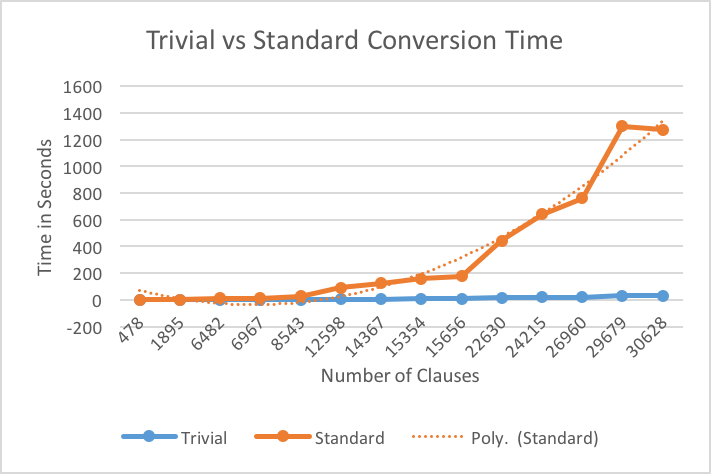
\includegraphics{png/trivialvsstandardconversiontime.png}
\end{center}

\begin{center}
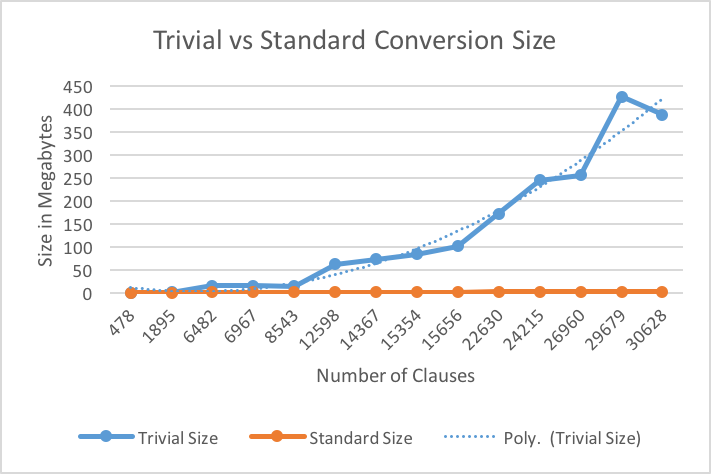
\includegraphics{png/trivialvsstandardconversionsize.png}
\end{center}

\chapter{DepQBF vs. \textit{qbftoepr} and iProver} \label{depqbfvsqbftoepr}

\section{\textit{qbftoepr} and iProver Results}

\begin{center}
\begin{tabular}{| l | S[table-format=4.4] | S[table-format=4.4] | S[table-format=4.4] | }
\hline
\multirow{2}{*}{\textbf{Name}} & \multicolumn{3}{|l|}{\textbf{Average Time in Seconds}} \\
\cline{2-4}
& \textbf{\textit{qbftoepr}} & \textbf{iProver} & \textbf{Total} \\
\hline
\texttt{toilet\_g\_02\_01.2} & 0.0043 & 0.0253 & 0.0296 \\
\texttt{toilet\_g\_04\_01.2} & 0.0043 & 0.0220 & 0.0263 \\
\texttt{toilet\_g\_08\_01.2} & 0.0046 & 0.0260 & 0.0306 \\
\texttt{toilet\_g\_20\_01.2} & 0.0156 & 0.0870 & 0.1026 \\
\hline
\end{tabular}
\end{center}

\section{DepQBF Results}

\begin{center}
\begin{tabular}{| l | S[table-format=3.2] |}
\hline
\textbf{Name} & \textbf{Average Time in Seconds} \\ \hline
\texttt{toilet\_g\_02\_01.2} & 0.0036 \\
\texttt{toilet\_g\_04\_01.2} & 0.0036 \\
\texttt{toilet\_g\_08\_01.2} & 0.0093 \\
\texttt{toilet\_g\_20\_01.2} & 0.0066 \\
\hline
\end{tabular}
\end{center}

\section{Graphs of Time}

\begin{center}
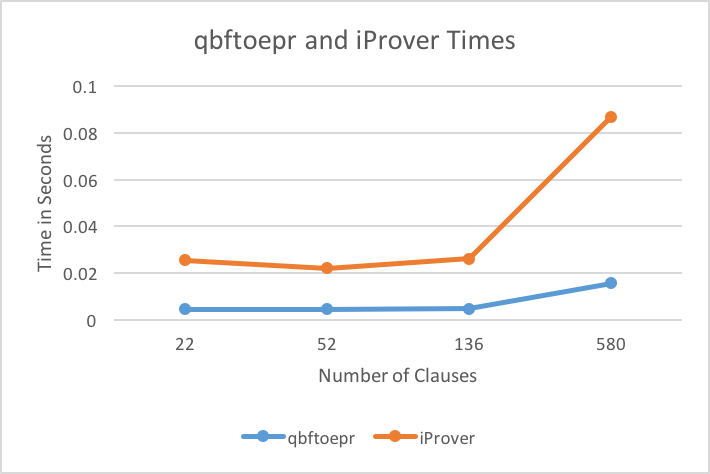
\includegraphics{png/qbftoeprandiprovertimes.png}
\end{center}

\chapter{\textit{qbftoepr} vs. qbf2epr} \label{qbftoeprvsqbf2epr}

\section{\textit{qbfoepr} Results}

\begin{center}
\begin{tabular}{| l | S[table-format=3.2] |}
\hline
\textbf{Name} & \textbf{Average Time in Seconds} \\ \hline
\texttt{s1196\_d3\_u} & 6.2243 \\
\texttt{s1269\_d3\_s} & 7.0686 \\
\texttt{s27\_d5\_u} & 0.0150 \\
\texttt{s298\_d11\_s} & 7.7326 \\
\texttt{s298\_d2\_s} & 0.0873 \\
\texttt{s298\_d5\_s} & 1.2313 \\
\texttt{s298\_d9\_s} & 4.9640 \\
\texttt{s386\_d12\_u} & 18.6606 \\
\texttt{s499\_d15\_s} & 29.1823 \\
\texttt{s499\_d4\_s} & 1.3090 \\
\texttt{s510\_d12\_s} & 30.6883 \\
\texttt{s510\_d4\_s} & 2.4000 \\
\texttt{s820\_d6\_s} & 14.9966 \\
\texttt{s820\_d7\_s} & 20.9876 \\
\hline
\end{tabular}
\end{center}

\begin{center}
\begin{tabular}{| l | S[table-format=3.2] |}
\hline
\textbf{Name} & \textbf{Average Time in Seconds} \\ \hline
\texttt{toilet\_g\_02\_01.2} & 0.0043 \\
\texttt{toilet\_g\_04\_01.2} & 0.0043 \\
\texttt{toilet\_g\_08\_01.2} & 0.0046 \\
\texttt{toilet\_g\_20\_01.2} & 0.0156 \\
\hline
\end{tabular}
\end{center}

\section{qbf2epr Results}

\begin{center}
\begin{tabular}{| l | S[table-format=3.2] |}
\hline
\textbf{Name} & \textbf{Average Time in Seconds} \\ \hline
\texttt{s1196\_d3\_u} & 0.5206 \\
\texttt{s1269\_d3\_s} & 0.5090 \\
\texttt{s27\_d5\_u} & 0.0410 \\
\texttt{s298\_d11\_s} & 0.5616 \\
\texttt{s298\_d2\_s} & 0.0676 \\
\texttt{s298\_d5\_s} & 0.1940 \\
\texttt{s298\_d9\_s} & 0.4213 \\
\texttt{s386\_d12\_u} & 1.0376 \\
\texttt{s499\_d15\_s} & 1.5356 \\
\texttt{s499\_d4\_s} &  0.1923\\
\texttt{s510\_d12\_s} & 1.5966 \\
\texttt{s510\_d4\_s} & 0.2506 \\
\texttt{s820\_d6\_s} & 0.8716 \\
\texttt{s820\_d7\_s} & 1.1506 \\
\hline
\end{tabular}
\end{center}

\begin{center}
\begin{tabular}{| l | c |}
\hline
\textbf{Name} & \textbf{Average Time in Seconds} \\ \hline
\texttt{toilet\_g\_02\_01.2} & 0.0546 \\
\texttt{toilet\_g\_04\_01.2} & 0.0353 \\
\texttt{toilet\_g\_08\_01.2} & 0.0370 \\
\texttt{toilet\_g\_20\_01.2} & 0.0473 \\
\hline
\end{tabular}
\end{center}

\chapter{Gantt Chart} \label{ganttchart}
\begin{center}
\begin{ganttchart}[
  vgrid={dotted, dotted, dotted, dotted, dotted, dotted, dotted, dotted, dotted, dotted, dotted,  dashed, dotted, dotted, dotted, dotted, dotted, dotted, dotted, dotted, dotted, dotted, dotted },
  hgrid,
  x unit = 0.39cm,
  y unit chart = 0.78cm,
  milestone label font=\bfseries
]{1}{24}
\gantttitle{Semester 1}{12}
\gantttitle{Semester 2}{12}\\
\gantttitlelist{1,...,12}{1}
\gantttitlelist{1,...,12}{1}\\

\ganttbar{Create plan}{1}{1}\\
\ganttbar{Learn OCaml}{1}{2}\\
\ganttbar{Handle Input}{2}{5}\\
\ganttbar{Prepare for Seminar}{6}{9}\\
\ganttmilestone{Seminar}{9}\\
\ganttbar{Skolemization}{6}{10}\\
\ganttbar{Removing Functions}{10}{12}\\

\ganttbar{Output TPTP}{13}{15}\\
\ganttbar{Prepare Results}{16}{17}\\
\ganttmilestone{Demonstration}{17}\\
\ganttbar{Optimizations}{15}{18}\\
\ganttbar{Finishing Touches}{19}{19}\\
\ganttmilestone{Code Deadline}{19}\\
\ganttbar{Report and Screencast}{20}{23}\\
\ganttmilestone{Final Deadline}{23}
\end{ganttchart}
\end{center}

\end{appendices}

\end{document}
